\section{Experiment and results}
In this chapter, we select the original model dynamic topic model(DTM)\cite{blei_dynamic_2006} as a baseline, and latest approach dynamic embedded topic model(DETM)\cite{dieng_dynamic_2019} to compare with our model.
\subsection{Experiment settings}
\paragraph{Datasets}
% First datasets, vocabularies, years 
We select the \textsc{un} debates as one of the testing corpus for the experiment. It is a collection of transcript from the official of UN member countries expressing about the  government's perspective over the world issues at the time.
After preprocessing, It contains 46 years time span of data, with 7507 documents and 6831 tokens in total. We selected 6005 for training, 1402 documents for testing and 100 documents for validation.
% Second datasets - NeurIPS 1987-2019
Second dataset we selected is NeurIPS conference paper dataset. The dataset contains conference papers ranged from 1987-2019. After preprocessing, it contains 9677 papers in total and 9182 tokens. Within the dataset, we pick 7345 documents for training, 1737 for testing and 100 for validation.
\paragraph{Data pre-processing}
To prepare the data sets for training, we pre-process the documents and turn them into useful corpus.
% Preprocess
We remove the special characters and stop words, perform tokenization. 
% three datas
In order to train the model, we have to leverage the data sets to feed-in different model. Specifically, three input data are to be generated to feed
% document-vocabularies
First, the bag-of-word $ w\in\mathbb{R}^{D\times V} $ is a matrix consist of the word count for vocabularies exist in every document. The document frequency for tokens are set to 100 documents minimum and 50\% at max.
% time-vocabularies
We also created a time-vocabularies word count matrix for the training of $ \eta $. The data set $ \tilde{w}\in\mathbb{R}^{T\times V} $ holds the word count for the vocabulary set over the time span $ t=1,\dots,T $.
% word sequence (seqlen=40)
For transformer embedding training, we alternate the data set into a sequence set $ S $ of equal distance of pre-defined sentence length $ \textsc{seqlen} $. Token $ \textsc{<empty>} $ are padded to the sequence when the sentence in i-index $ S[i]<\textsc{seqlen} $. The sequence data set are to train the transformer embedding as input in the training process.
% DTM, DETM, our model
\paragraph{Models}
% TODO
For D-ETM model, we follow the default settings instructed in \cite{dieng_dynamic_2019}. We set the variance of  on the prior to 0.005.
\paragraph{Algorithm configurations}
% alpha	
Following the parameter settings from \cite{blei_dynamic_2006}, the variance of prior in $  $ are set to $ \gamma^2=0.005 $ on $ \alpha\sim\mathcal{N}(\cdot,\cdot) $.
% transformer
We set the dimension for the transformer embedding is 256, and so for the hidden dimension for both transformer encoder and decoder. Each transformer encoder and transformer decoder consist of two layers and 2 heads for scaled dot-product. The sequence length the transformer are set to 40.
% gaussian process
For the gaussian process latent variable model, we selected zero mean with squared exponential function (RBF kernel) as the covariance prior, which allows providing adaptive change on topic-proportion against the possible rapid topic changes from documents. We follow the setting from \cite{tomasi_stochastic_nodate} and set the length scale of kernel as 0.1.
\subsection{Results}
\paragraph{Training}
In the training stage, we perform black box variational inference to estimate the unbiased gradient estimator with Monte Carlo sampling for intractable variational lower bound.
\paragraph{Quantitative results}
The result of models are to compare in terms of perplexity, Topic Coherence (TC), Topic Diversity (TD). To calculate the topic coherence and topic diversity, we average down the scores over time span $ 1\dots T $.
% table for perplexity, topic coherence, and topic diversity
\begin{table}[h]
\centering
\begin{tabular}{llll}
\hline
     & Perplexity  &TC&TD\\ \hline
D-LDA	     	&  pending & pending&pending\\
D-ETM	     	&  3050.5 & pending&0.1996\\
\textbf{Our model}  & 5139.5 & 0.129& 0.749\\ \hline
\end{tabular}
\captionof{table}{Result on UN debates dataset, k=50\label{tbl:ch6_t1}}
\end{table}
\begin{table}[h]
\centering
\begin{tabular}{llll}
\hline
     & Perplexity  &TC&TD\\ \hline
D-LDA	     	&  pending & pending&pending\\
D-ETM	     	&  pending & pending&pending\\
\textbf{Our model}  & 5387.9 & 0.159& 0.611\\ \hline
\end{tabular}
\captionof{table}{Result on NeurIPS dataset (1987-2019), k=20\label{tbl:ch6_t2}}
\end{table}
From table \ref{tbl:ch6_t1}, we have compared our model with the latest model. On the UN debate data set, we conduct the experiment with number of topic $ k=50 $. In terms of perplexity, the D-ETM model has performed a better score. On the other hand, our model obtain a better performance in terms of topic coherence and topic diversity, which is 0.129 and 0.749 respectively. 
\subsubsection{Qualitative results}
% visualization for the documents by topics
\paragraph{UN debates}We put the document-topic proportion obtained from the model and run t-SNE algorithm to transform the document-topic proportion into 2-dimensional continuous space. Shown in figure \ref{fig:tsne1}, different colors of dots represent a specific topic. As can be seen, apparently the documents can be classified in to interpretable cluster according to their topic.\\
\begin{figure}[h]
\centering
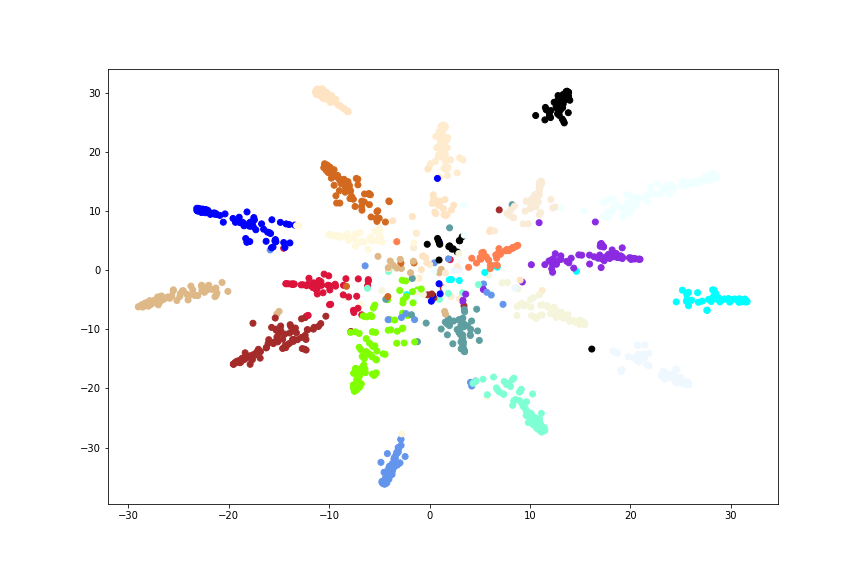
\includegraphics[width=0.9\linewidth]{figures/1128/tsne1}
\caption{Visualization for document}
\label{fig:tsne1}
\end{figure}
% Scatter visualization for the words over time
From the result we obtained, we select top-6 topics have the highest proportion to the document set and display them on figure \ref{fig:scatter}. And for those topics, we extract top-5 words having the highest proportion. Then we track those words how they change their proportion to the corresponding topic. As demonstrated, the topic words in each topic selected doesn't diverse each other very much in proportion, resulted a coherent trend that the word are more likely adhere to the topic.\\
% add specific information, what can you see from the word on some topic
\begin{figure}[h]
\centering
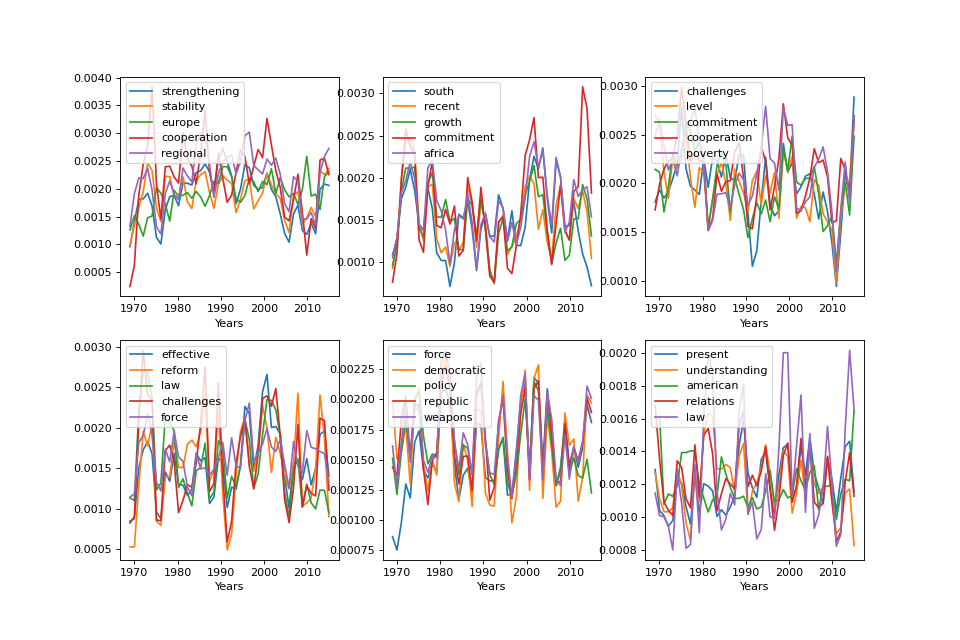
\includegraphics[width=0.9\linewidth]{figures/1128/scatter}
\caption{word trends over time (UN debates)}
\label{fig:scatter}
\end{figure}
% topic over time representation
Accordingly, in figure \ref{fig:stack} we also track the change of those topic over time. Different color in the cumulative graph represents the topics evolve along the time period. \\
% Specific: explain what you saw from the topic trend
\begin{figure}[h]
\centering
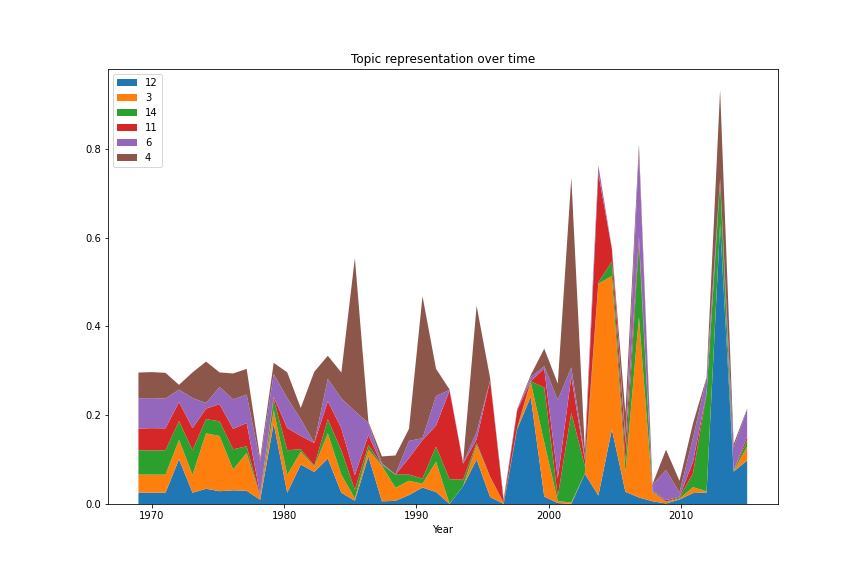
\includegraphics[width=0.9\linewidth]{figures/1128/stack}
\caption{Topic trend in top-6 topics (UN debate)}
\label{fig:stack}
\end{figure}
% NeurIPS
\paragraph{NeurIPS dataset} % we put k=20 into experiment setting
To investigate the word trends change over time, table \ref{tbl:ch6_t3} visualize the words by 5 years interval. In particular, we selected a topic corresponding to reinforcement learning and pick top-10 words for each time stamp. By observation, we see that the topic are coherent in several keywords like \textsc{control}, \textsc{action} and \textsc{state}. On the other hand, some other keywords also highlight their importance upon specific time period. For instance, words like \textsc{markov}, \textsc{policy} and \textsc{discount} are more likely to appear before; word \textsc{reinforcement} appears since 2012. For sake of interpretability, we also highlight the first appearance in the year for those keywords related to reinforcement learning.
% Figure word trend
On figure\ref{fig:scatter2}, displays the word trend from top-6 topics over the time. We have selected 3 representative tokens from top-10 words for each topic. And observe how the words trends though the years. 
% Topic trend over time
On figure \ref{fig:stack2}, we provide a stack plot for how those top-6 topics changed over time. Apparently it demonstrates how the topics are inclining or declining. For example, the topic related to .. is gaining more popularity over time. Besides, the topic about .. is being less important by the years.
\begin{table}[h]
\centering
\begin{tabular}{ll}
\hline
Year&Topic: Reinforcement Learning\\ \hline
1987 &\hl{control} position world simulated initial \\
&search change \hl{environment} modification \hl{action}\\
1992 &temporal watkins cambridge dynamic controller \\
&sutton \hl{states} control actions action\\
1997 &states actions \hl{markov} \hl{decision} control \\
&dynamic \hl{discount} action discounted \hl{policy}\\
2002 &\hl{transition} decision dynamic \hl{reward} markov \\
&policies states actions policy action\\
2007 &artificial intelligence rewards policies programming \\
&states action reward actions policy\\
2012 &\hl{reinforcement} decision markov states mdp \\
&action policies reward actions policy\\
2017 &action markov policies reinforcement transition \\
&expected control states policy reward\\
\hline
\end{tabular}
\captionof{table}{Word trend in topic reinforcement learning (5 years interval)\label{tbl:ch6_t3}}
\end{table}
\begin{figure}
\centering
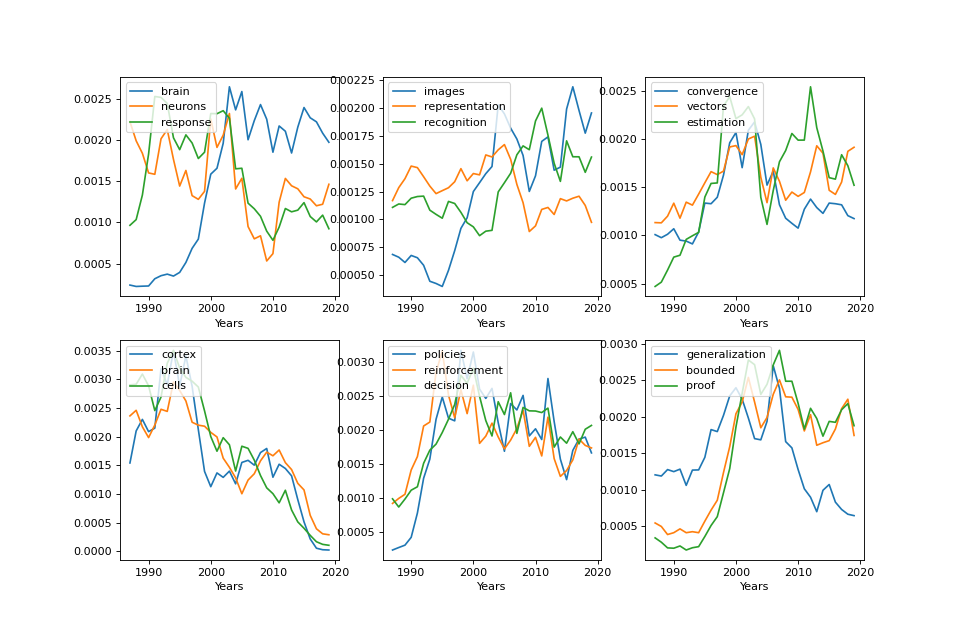
\includegraphics[width=1\linewidth]{figures/1128/scatter(2)}
\caption{Word trend for top-6 topics (NeurIPS dataset)}
\label{fig:scatter2}
\end{figure}
\begin{figure}
\centering
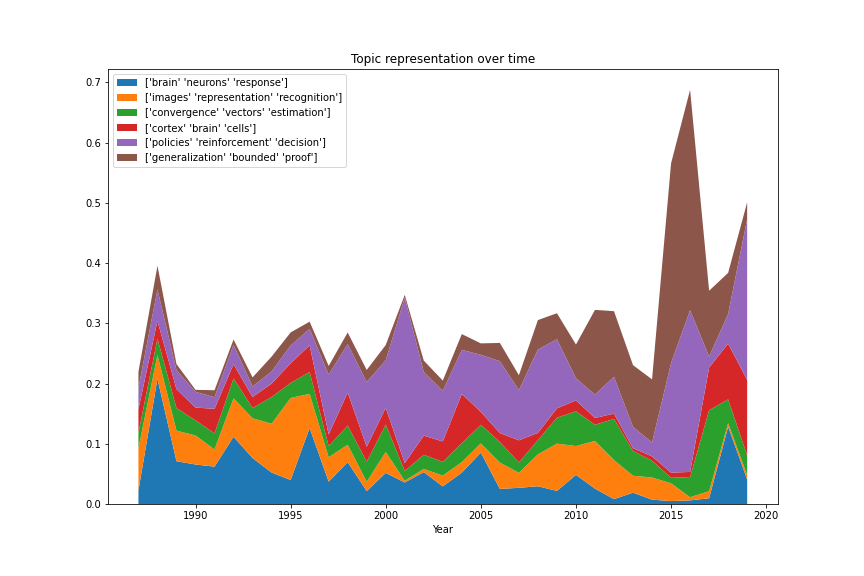
\includegraphics[width=1\linewidth]{figures/1128/stack(2)}
\caption{Topic trend for top-6 topics (NeurIPS dataset)}
\label{fig:stack2}
\end{figure}
% Discussion
\subsubsection{Discussion}
In the result, we observe that our model has been out perform the D-ETM model in TC and TD scores. Apparently the topic words in our model generated are coherent over time and consistent 